% !TeX root = ../../../Main.tex

\chapter{Function Approximation}
\label{chapter4}

A common problem in engineering is developing a model from measurement data. Such a model makes it possible to generalize from the given data to new data where a real measurement does not exist. The process of developing a model is often combined with function approximation. The goal here is to find a mapping as a linear combination of elements, which constitute a basis from functions, that approximates a given behavior, also called a target function, as close as possible.

Mathematically, function approximation is the process of finding a mapping from inputs $x$ to outputs $y$. Usually, a set of $x_{fit}$ and corresponding $y_{fit}$ is given and the goal is to find a function that returns a value close to $y_{fit,i}$ for each $x_{fit,i}$.

There are two types of function approximation. In some cases, knowledge about the specific problem can help to find suitable base functions. If, for example, a mapping is known to be linear ($y=a_0 + a_1 x$), the function approximation process degenerates to finding the two coefficients $a_0$ and $a_1$. The same applies to quadratic, trigonometric or exponential target functions or linear combinations of them. If, however, the target function is not known, function approximation is more elaborate. One can try multiple target functions or combine them in order to find one, that fits best, or use a \textit{universal function approximator} like an artificial neural network. 

\section{Tables}

The simplest way to express a discrete mapping is by a table where each input/output pair is represented by a cell of the table. The number of inputs and corresponding outputs in a table is inherently finite. The set of states and actions in a continuous MDP is however infinite, so the policy and value functions must also be continuous. If a discrete mapping like a table is used as a representation of a policy or value function in a continuous MDP, it will, at some point, be confronted with unknown inputs. The inability to deal with unknown inputs is a big disadvantage of tables. There are, however, ways to overcome this weakness.

A written version of the value function table and the table containing the greedy action for each state can be found in appendix \ref{appendix_C}.

\subsubsection{Nearest Neighbor}

The most straightforward way to obtain an output for an unknown input is to look for the table entry that is closest to the unknown input. This yields a piecewise constant mapping from inputs to outputs and enables the table to generalize. Whether this suffices as an approximation for a continuous mapping $f$ heavily depends on the properties of $f$ . If there are large differences between the output of two subsequent inputs, the error can be quite high.

\subsubsection{Linear Interpolation}

Another way to obtain outputs for unknown inputs is to interpolate linearly. In a first step, the two nearest known inputs $x_0$ and $x_1$ and their respective outputs $y_0$ and $y_1$ are looked up (note that $x_0 \leq x \leq x_1$ in this case). In the second step, the output is calculated by the following formula:

\begin{equation}
y_{interp} = y_0 \cdot (1-\gamma) + y_1 \cdot \gamma
\end{equation}

where $\gamma = \frac{x - x_0}{x_1 - x_0}$.

One advantage of linear interpolation of table values is that the output is at least continuous, though not differentiable at the known input points.

\section{Artificial Neural Networks}

The structure of artificial neural networks resembles the structure of a human brain according to the current state of research \cite[Chapter~1.1]{Kriesel2007NeuralNetworks}. The human brain consists of a very high number of neurons, each receiving signals from other neurons, processing them and itself sending a signal to other neurons if certain conditions are met. Each neuron is very simple, it is the high number of them and the fact that they all work in parallel that makes the human brain so powerful. 

\begin{figure}[h]
	\centering
	\tikzsetnextfilename{neuron}	
	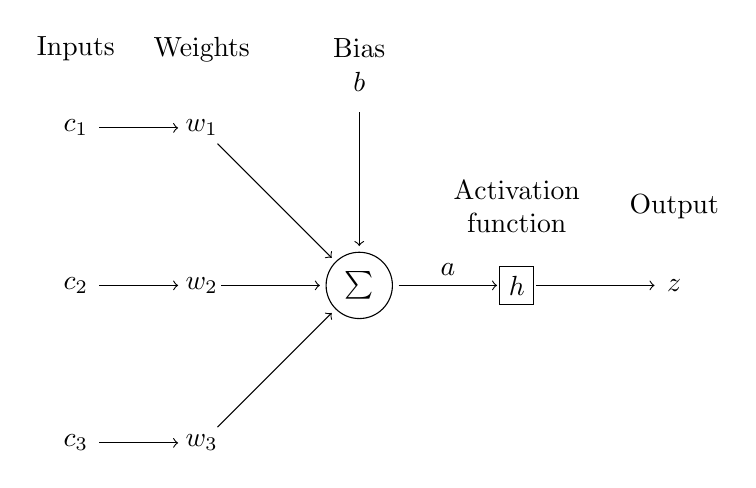
\begin{tikzpicture}
	
	\pgfplotsset{
		width=0.8\textwidth,
		height=0.9\textwidth, 
		xmajorgrids, 
		ymajorgrids, 
		enlarge x limits=false,
		scaled x ticks = false,
		x tick label style={/pgf/number format/.cd, fixed, set thousands separator={}},
		scaled y ticks = false,
		yticklabel style={/pgf/number format/.cd, fixed, set thousands separator={}},
		xmin=0, xmax=6,
		legend pos=north west,
		legend cell align=left
	}
	\node[circle, draw=black, fill=white] at (0,0) {$\sum$};
	\node at (-3.6,3) {Inputs};
	\node at (-2,3) {Weights};
	\node[text width=4cm,align=center] at (2,1) {Activation \\ function};
	\node[align=center] at (4,1) {Output};
	\node at (-3.6,2) {$c_1$};
	\node at (-3.6,0) {$c_2$};
	\node at (-3.6,-2) {$c_3$};
	\node at (-2,2) {$w_1$};
	\node at (-2,0) {$w_2$};
	\node at (-2,-2) {$w_3$};
	\node[text width=1cm,align=center] at (0,2.8) {Bias \\ $b$};
	\node[draw=black] at (2,0) {$h$};
	\node at (4,0) {$z$};
	\draw[->] (-1.8,1.8) -- (-0.35,0.35);
	\draw[->] (-1.75,0) --  (-0.5,0);
	\draw[->] (-1.8,-1.8) -- (-0.35,-0.35);
	\draw[->] (0,2.2) -- (0,0.5);
	\draw[->] (0.5,0) -- node [above] {$a$} (1.75,0);
	\draw[->] (-3.3,0) -- +(1,0);
	\draw[->] (-3.3,2) -- +(1,0);	
	\draw[->] (-3.3,-2) -- +(1,0);
	\draw[->] (2.25,0) -- +(1.5,0);
	
	\end{tikzpicture}
	\label{tikz:neuron}
	\caption{A neuron in an artificial neural network}
\end{figure}

A neuron in an artificial neural network looks like what is depicted by Fig. \ref{tikz:neuron}. It takes an arbitrary number of inputs $c_i$, multiplies each input by the corresponding input weight $w_i$, adds a bias and applies to the result $a$ a nonlinear function, the so called activation function $h$, yielding $z$, the neuron output. This output can either serve as an input to another neuron or as the network output. Multiple activation functions are common, but they all are somewhat s-shaped. Most activation functions map the set of real numbers to the range between $-1$ and $1$ or sometimes between $0$ and $1$, limiting the neuron output and therefore its influence on the output of the ANN network. Examples include the step function, ($z=1$ if $x \geq x_0$, $z=0$ otherwise), the rectifier nonlinearity ($h(x)=\max(0,x)$), the sigmoid function ($h(x)=1/(1+e^{-x})$) and the tanh-activation function ($h(x)=\tanh(x)=\frac{e^x-e^{-x}}{e^x+e^{-x}}$).
Nonlinearity is essential here, because if linear activation functions are used, each neuron output is a linear function of its inputs. Any combination of linear mappings is itself linear. So if a deep neural network has only linear activation functions, the ANN output is always a linear function of the inputs, regardless of the number of hidden layers. Therefore, a deep neural network, where all activation functions are linear, does not make sense.

\begin{figure}[h]
	
\includegraphics[width=\textwidth]{src/pics/dummy.jpg}
	\caption{Activation functions \cite{Zuern2017}}
	\label{fig:activation_functions} 
\end{figure}

In an artificial neural network, the neurons are arranged in layers. The ANNs in this work are all fully connected feed forward networks, also known as Multi Layer Perceptrons (MLPs)\nomenclature[A]{MLP}{multi layer perceptron}. Each neuron in a given layer $k$ gets an input from each neuron in the previous layer $k-1$ and outputs a signal to each neuron in the next layer $k+1$ (see figure \ref{fig:neuron}).

\begin{figure}[h]
	\centering
	\tikzsetnextfilename{MLP}	
	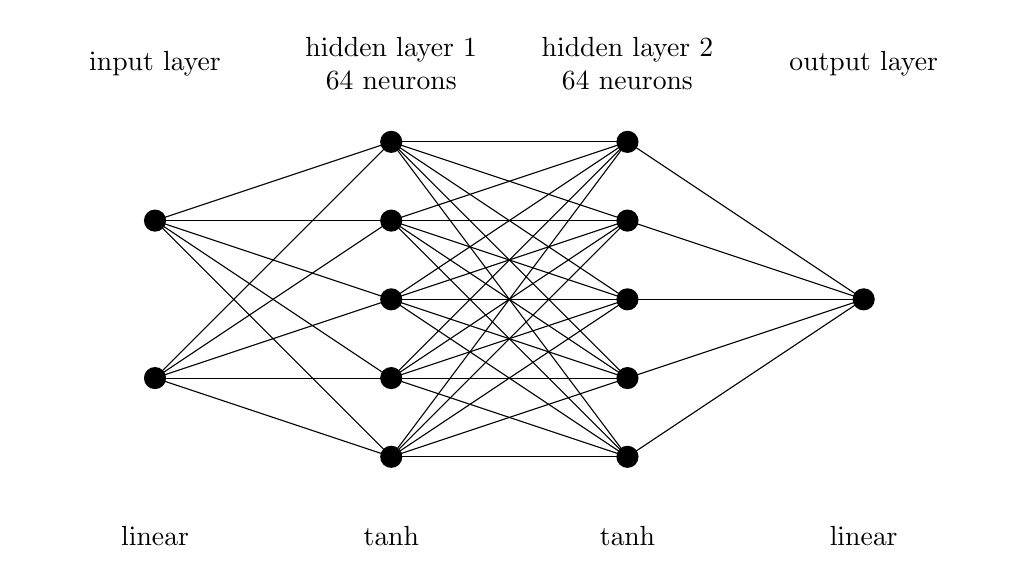
\begin{tikzpicture}
	
	\pgfplotsset{
		width=0.8\textwidth,
		height=0.9\textwidth, 
		xmajorgrids, 
		ymajorgrids, 
		enlarge x limits=false,
		scaled x ticks = false,
		x tick label style={/pgf/number format/.cd, fixed, set thousands separator={}},
		scaled y ticks = false,
		yticklabel style={/pgf/number format/.cd, fixed, set thousands separator={}},
		xmin=0, xmax=6,
		legend pos=north west,
		legend cell align=left
	}
	
	
	\fill[black] (2,-2) circle (4pt) ;
	\fill[black] (2,-0) circle (4pt) ;
	\fill[black] (5,-3) circle (4pt) ;
	\fill[black] (5,-2) circle (4pt) ;
	\fill[black] (5,-1) circle (4pt) ;
	\fill[black] (5,0) circle (4pt) ;
	\fill[black] (5,1) circle (4pt) ;
	\fill[black] (8,-3) circle (4pt) ;
	\fill[black] (8,-2) circle (4pt) ;
	\fill[black] (8,-1) circle (4pt) ;
	\fill[black] (8,0) circle (4pt) ;
	\fill[black] (8,1) circle (4pt) ;
	\fill[black] (11,-1) circle (4pt) ;

  	\foreach \a in {-2,0}
  		\foreach \b in {-3,-2,-1,0,1}
			\draw (2,\a) -- (5,\b);
	
  	\foreach \c in {-3,-2,-1,0,1}
		\foreach \d in {-3,-2,-1,0,1}
			\draw (5,\c) -- (8,\d);
			
			
	\foreach \e in {-3,-2,-1,0,1}
			\draw (8,\e) -- (11,-1);
	
	\node[text width= 3cm,align=center] at (2,2) {input layer};
	\node[text width= 3cm,align=center] at (5,2) {hidden layer 1 \\ 64 neurons};
	\node[text width= 3cm,align=center] at (8,2) {hidden layer 2 \\ 64 neurons};
	\node[text width= 3cm,align=center] at (11,2) {output layer};

	\node[text width= 3cm,align=center] at (2,-4) {linear};
	\node[text width= 3cm,align=center] at (5,-4) {tanh};
	\node[text width= 3cm,align=center] at (8,-4) {tanh};
	\node[text width= 3cm,align=center] at (11,-4) {linear};
	
	\end{tikzpicture}
	\label{tikz:MLP}
	\caption{The MLP used for the policy}
\end{figure}

If a policy or value function is represented by an artificial neural network (ANN\nomenclature[A]{ANN}{Artificial Neural Network}), the output for each state (or state-action-pair) is determined by the weights and biases of the network and the activation functions. As the latter are usually given or predetermined (and not trained), only the weights and biases are regarded as parameters. One set of weights and biases forms the \textit{parameter vector} $\theta$ of the neural network. If, for example, a stochastic policy is parametrized by $\theta$ and represented by a neural net with $k$ layers, the notation is as follows:

\begin{equation}
\pi_\theta(a|s)=\mathbb{P}[a|s,\theta]
\end{equation}

with

\begin{equation}
\theta = \{\boldsymbol{W}^{(1)},\boldsymbol{b}^{(1)},\boldsymbol{W}^{(2)},\boldsymbol{b}^{(2)}, ...,
\boldsymbol{W}^{(k)},\boldsymbol{b}^{(k)}\}
\label{eq:theta}
\end{equation}

The policy ANN does not necessarily need to output the action directly. Instead, most RL-related policies are stochastic, i.e. the neural net outputs the mean and standard deviation of a normal distribution:

\begin{equation}
\pi_\theta(\mu_\theta,\sigma_\theta|s)=\frac{1}{\sqrt{2\pi}\sigma_\theta}e^{-\frac{(a-\mu_\theta)^2}{2\sigma_\theta^2}}
\end{equation}

The action $a$ is then drawn from $\mathcal{N}(\mu_\theta(s),\sigma^2_\theta(s))$. 
In this work, the policy is represented with a neural network that has two outputs, the mean and standard deviation. Dynamic Programming is used only to find the optimal mean values. The standard deviation is set to 0.5. This serves as an intial solution for the policy net to be trained by an RL method.

\subsection*{Input Standardization}

All training algorithms that are used in this work rely on the partial derivative of a loss function with respect to the network weights and biases. As can be seen in \ref{eq:gd_update} and the following equations, they perform a step in (an approximation of) the current gradient direction. This gradient heavily depends on the network inputs. If some of the inputs have much larger values than the rest, this can result in some weights being updated faster than others, which is not desirable. Therefore, the inputs to a neural network should have the same scale. In this work, the inputs are scaled to a normal distribution with $\mu = 0$ and $\sigma = 1$:

\begin{equation}
\hat{x} = \frac{x - \mu}{\sigma}
\end{equation}

The specific values for $\mu$ and $\sigma$ for each of the scenarios are presented in table \ref{tab:glider_data}.

\subsection*{Action Scaling}

In an artificial neural network, every neuron can output a value between -1 and 1. Therefore, the output of a neural network is limited by the number of neurons in the last hidden layer. Obtaining a large output requires a lot of neurons. On the other hand, lots of neurons favor overfitting and increase training time. If the desired outputs are too small, then so are the neuron outputs. The $tanh(\cdot)$ activation function that is used for the policy is approximately linear in this area. Therefore the whole network behaves almost linearly if it is trained to output values close to zero and linear behavior can also be obtained without any hidden layers. The most important advantage of deep neural networks is however their ability to represent highly nonlinear behavior.

Both problems can be avoided if outputs lie between -1 and 1. This way it is unlikely that any of the activation functions reach their saturation limit, nor is the network restricted to linear behavior. Therefore, the neural network is usually trained to output values between -1 and 1 and these values are then scaled to the desired magnitude by multiplying them with a scaling factor. Another way to mitigate this problem is choosing activation functions that are also nonlinear if the input is close to zero.

\subsection*{Weight initialization}

Training an artificial neural network is an iterative process. Therefore it requires initial values for the weights and biases. As training a neural network through supervised learning comes down to solving an optimization problem iteratively, training success highly depends on the initial weights.

The two most popular ways to initialize neural network weights are the Glorot uniform initialization and the glorot normal distribution. According to the glorot uniform initialization, the weights in one layer must be distributed uniformly within $\pm \sqrt{\frac{6}{n_{in}+n_{out}}}$ where $n_{in}$ and $n_{out}$ are the numbers of neurons in the prior and current layer, respectively.

The Glorot normal initialization states that the weights must be initialized according to a normal distribution with zero mean and a variance of $\sigma = \sqrt{\frac{2}{n_{in}+n_{out}}}$.

In this work, all neural networks are initialized according to the Glorot uniform distribution. 

\section{Supervised Learning}
All machine learning algorithms can be divided into two categories: supervised learning and unsupervised learning. In supervised learning, the agent is given the desired action for each state explicitly, so it knows what it is supposed to do. In unsupervised learning, however, the agent does not know what the best action is, so it has to find out itself. One way of doing that is from moving in the state space and learning from experience, for example by applying a reinforcement learning algorithm.

In the supervised learning case, training is done via minimizing a loss function that depends on the desired action and the actual action taken by the agent. A common loss-function is the mean squared error (MSE)\nomenclature[A]{MSE}{mean squared error}:

\begin{equation}
L = \frac{1}{N}\cdot\sum_{n=1}^{N}L_n =  \frac{1}{N}\cdot\sum_{n=1}^{N}[\frac{1}{2}\cdot(a_n(s)-a_{n,fit})^2]
\label{lossfun}
\end{equation}

The goal of supervised learning is to minimize the difference between $a_{n,fit}$ and $a_n(s)$ in each state. If $a_n(s)$ is the output of a function approximator, minimizing $L_{MSE}$ is equivalent to fitting the function approximator to the desired outputs.

One advantage of the application of a loss function is that numerous iterative optimization algorithms have been developed to solve such a problem.

\section{Optimization Techniques}

As mentioned before, supervised learning is usually done by defining a loss function that depends on the network weights and biases and finding a local or global minimum numerically.

In this work, the ADAM algorithm is used for training the policy to output the desired action at each point in the state space. As most optimization algorithms, ADAM is gradient-based. Therefore, some insight into the general ideas behind gradient based numeric optimization is useful for understanding ADAM. Sections \ref{sec:grad_desc} and \ref{sec:sgd} explain briefly how gradient based optimization works in general. In section \ref{sec:adam}, ADAM is described and explained.

All presented algorithms produce a series of points in the space that the network weights and biases establish. The point at the k-th optimization step is defined by a distinct set of weights and biases $\theta$, similar to coordinates in the state space (c.f. Eq. \ref{eq:theta}).

\subsection{Gradient Descent}
\label{sec:grad_desc}

In gradient descent, the next point $\theta_{k+1}$, i.e. the next set of weights and biases, is reached by computing the gradient of the loss function with respect to the network weights, $\nabla_{\theta_k}L_k$, and performing one step in the direction of steepest descent. $\theta_{k+1}$ is calculated by the following equation:

\begin{equation}
\theta_{k+1} = \theta_k - \nabla_{\theta_k}L_k\cdot \alpha
\label{eq:gd_update}
\end{equation}
with
\begin{align}
\nabla_{\theta_k}L_k &=\frac{1}{N}\cdot\sum_{n=1}^{N}\nabla_{\theta_k}L_{n,k} \\
&=\frac{1}{N}\cdot\sum_{n=1}^{N}[(a_n(s)-a_{n,fit})\cdot\nabla_{\theta_k}a_n(s)]
\end{align}
and an arbitrary step size $\alpha$.

The choice of $\alpha$ has a big effect on the convergence of the optimization algorithm. If $\alpha$ is too small, each $\theta_{k+1}$ is close to the respective $\theta_{k}$ so it takes many steps to find a minimum. If $\alpha$ is too big, the algorithm might not converge at all.

Ordinary gradient descent methods are not suitable for optimizing the output of large artificial neural networks because computing the gradient $\frac{\partial L_k}{\partial \theta_k}$ for all the weights and biases is very computation-intensive and time-consuming.

\subsection{Stochastic Gradient Descent}
\label{sec:sgd}

As mentioned before, the output of a neural network cannot be optimized efficiently with a gradient descent algorithm. One way to bypass this weakness is Stochastic Gradient Descent (SGD). If the loss function is a sum like in Eq. \ref{lossfun}, it is sufficient to calculate the gradient of only one summand of the loss function, i.e. only consider one random training sample at each step $k$, and perform a small step in the corresponding direction:

\begin{equation}
\nabla_{\theta_k}L_k \approx \nabla_{\theta_k}L_{n,k}
\label{sgd_gradient}
\end{equation}

\begin{equation}
\theta_{k+1} = \theta_k - \nabla_{\theta_k}L_{n,k} \cdot \alpha
\label{sgd_update}
\end{equation}

If this is done for all samples successively, it also converges to the loss from Eq.\ref{lossfun}. 
Thanks to the faster computation of $\nabla_{\theta_k}L_{n,k}$, SGD converges faster than ordinary gradient descent although Eq.\ref{sgd_gradient} is only a rough estimate of the true gradient.


\subsection{The ADAM Algorithm}
\label{sec:adam}

Basic Stochastic Gradient Descent has a fixed stepsize $\alpha$. Most advanced optimization algorithms have a variable stepsize and an update direction that depends on the previous updates to accelerate convergence. One example is to add a momentum term to the gradient from Eq.\ref{sgd_update}. This affects the step size and the direction of the update.

It takes into account the previous update and changes the direction of the next update. Like a ball rolling down a slope, the algorithm does not immediately change direction if the gradient of the slope changes direction or stop if the gradient is zero. If there is a plateau in the loss function or a weak local minimum, ordinary algorithms tend to get stuck there. With momentum, the risk of getting stuck is reduced.

The ADAM-algorithm utilizes a modified momentum term for better convergence. Equation \ref{eq:adam_update} shows one update step, the parameters $\hat m_t$ and $\hat v_t$ are calculated with equations \ref{eq:adam_hat_m} and \ref{eq:adam_hat_v}.

\begin{equation}
\theta_{k+1}=\theta_k-\alpha\cdot\frac{\hat{m}_t}{\sqrt{\hat v_t}+\epsilon}
\label{eq:adam_update}
\end{equation}

with

\begin{equation}
\hat{m}_t= \frac{m_t}{1-\beta_1^t}= \frac{\beta_1\cdot m_{t-1}+(1-\beta_1)\cdot g_t}{1-\beta_1^t},
\label{eq:adam_hat_m}
\end{equation}


\begin{equation}
\hat v_t= \frac{v_t}{1-\beta_2^t}= \frac{\beta_2\cdot v_{t-1}+(1-\beta_2)\cdot g_t^2}{1-\beta_2^t}
\label{eq:adam_hat_v}
\end{equation}

The algorithm utilizes the first and second moments of the previous gradients to calculate the update. Consider a pair of $m_t$ and $v_t$ that follow recursively from $m_{t-1}$ and $v_{t-1}$ according to equations \ref{eq:adam_hat_m} and \ref{eq:adam_hat_v}. For the calculation of each $m_t$ and $v_t$, the previous value $m_{t-1}$ and the current gradient $g_t$ are used. $m_t$ and $v_t$ are biased estimates of the first and second moments, there is a correction term in each of the denominators of equations \ref{eq:adam_hat_m} and \ref{eq:adam_hat_v} to account for that. See \cite{DBLP:journals/corr/KingmaB14} for more details.

\section{Overfitting}

It is seldom desirable to minimize the loss function to its absolute minimum value on the training data. At first, this might sound counterintuitive. But apart from the additional time it takes to get there, it increases the chances of running into problems.

When dealing with a continuous state space, it is common practice to discretize it and deal with the discretized state space instead. While a continuous state space consists of an infinite number of states, the number of states in the discretized state space is finite. This reduces computation time and makes some algorithms applicable in the first place. If an appropriate grid is used (i.e. if it is dense enough in relevant areas of the state space), the solution is likely to be close to the solution of the continuous problem. The more grid points, the closer the solution is to the continuous solution.

If, however, a function approximator like an ANN is optimized on the discretized state set, it is possible that, although it might fit the training data very closely, it may not generalize well, i.e. give unexpected outputs when fed with states that have not been used in training. This problem is called \textit{overfitting}. It especially occurs if at least one of the following conditions is met:

\begin{itemize}
	\item Noisy data (every data point differs slightly from the expected value)
	\item Limited dataset (only a few points to fit to)
	\item High number of parameters (many degrees of freedom)
\end{itemize}


\begin{figure}[h]
	\centering
	\pgfplotstableread[col sep=comma] {\detokenize{./src/pics/tikz/overfitting_plot.dat}}\overfittingdat
	
	\tikzsetnextfilename{overfitting}
	
	\begin{tikzpicture}
	
		\pgfplotsset{
			width=0.8\textwidth,
			height=0.5\textwidth, 
			xmajorgrids, 
			ymajorgrids, 
			enlarge x limits=false,
			scaled x ticks = false,
			x tick label style={/pgf/number format/.cd, fixed, set thousands separator={}},
			scaled y ticks = false,
			yticklabel style={/pgf/number format/.cd, fixed, set thousands separator={}},
			xmin=0, xmax=6,
			legend pos=north west,
			legend cell align=left
		}
		
		\begin{axis}[
		% hide x-axis once
		% grid andeuten (andere Farbe)
		clip mode=individual,
		ymin=0, ymax=10,
		axis y line*=left,
		xlabel={x},
		xlabel near ticks,
		ylabel={y},
		ylabel near ticks,
		]
		
		\fill[black] (0,0.9) circle (2.5pt) ;
		\fill[black] (0.5,1.2) circle (2.5pt) ;
		\fill[black] (2,1.3) circle (2.5pt) ;
		\fill[black] (3.5,2.3) circle (2.5pt) ;
		\fill[black] (4,2.75) circle (2.5pt) ;
		\fill[black] (5,3.7) circle (2.5pt)  ;
		\fill[black] (6,4.4) circle (2.5pt)  ;
		% aircraft trajectory
		\addplot[red, line width=1.2pt, mark=none,forget plot] table[x index=0, y index=1]{\overfittingdat};
		\addplot[blue, line width=1.2pt, mark=none,forget plot] table[x index=0, y index=2]{\overfittingdat};
		
		\addlegendimage{red,line width=1.2pt, mark=none}\addlegendentry{10th order polynomial}
		\addlegendimage{blue,line width=1.2pt, mark=none}\addlegendentry{2nd order polynomial}
		
		\end{axis}
		
	\end{tikzpicture}
	\label{tikz:overfitting}
	\caption{Overfitting in case of a high order polynomial}
\end{figure}

Overfitting is an issue in many function- and curve-fitting applications. Fig. \ref{tikz:overfitting} shows overfitting in case of a high order polynomial. Although it is much simpler than a neural network, the problems are similar.

The plot shows two polynomials that have been fitted to a set of seven points. The blue line represents a quadratic polynomial, the red line belongs to a 10th order polynomial. A n-th order polynomial has n+1 parameters and can therefore be fit exactly to n+1 points. The quadratic polynomial only has three parameters and can therefore not pass through all seven points exactly. In such cases, fitting is done by minimizing the mean quadratic fitting error: 

\begin{align}
\bar{e}_{fit}&=\frac{1}{m}\sum_{i=1}^{m}[y_i-y_{i,fit}]^2 \\
&=\frac{1}{m}\sum_{i=1}^{m}[y_i-\sum_n (a_n\;x^n)]^2
\label{eq:overfitting_fitting}
\end{align}

where m is the number of given points. 

The 10th order polynomial has eleven parameters. It is therefore possible to fit the function exactly to the seven input points. This can be done by solving a system of linear equations where each point contributes one equation. In the case of the 10th order polynomial, there are eleven parameters. If this polynomial is fitted to seven points, there are seven equations and eleven parameters to be determined. The corresponding system of equations is called \textit{underdetermined}. Four of the parameters have to be set prior to solving the linear system. Their choice is arbitrary, which can lead to a shape like the red plot. Although the seven conditions at the points are met exactly, the blue plot intuitively seems like a more appropriate approximation.

Of course, any high order polynomial can also be fitted to a set of points by minimizing \ref{eq:overfitting_fitting}. Unfortunately, this can also lead to overfitting, because it uses the same information (input point coordinates). Therefore, it will eventually find a set of parameters that fits the points exactly and is likely to have the same oscillations as the red line shown in Fig. \ref{tikz:overfitting}.

In any application where there are more parameters than points to fit, overfitting can be an issue. Any function approximator should therefore only have as many parameters as necessary. Any additional parameter can increase the risk of overfitting. There are several other precautions that can be taken in order to avoid overfitting. Some of them are presented in the following paragraphs. \bigbreak


One way to deal with overfitting is splitting the state set into a set of training data and a set of validation data. After training on the training dataset, the value of the loss function on the training data is compared to the value of the loss function on the validation data. If - from one training step to the next - the training loss decreases while the validation loss does not, overfitting is likely. This can be used as a criterion to stop the training. Fig. \ref{tikz:overfitting_stop} shows how training loss and validation loss typically evolve during training. After iteration 63, only the training loss decreases. At this point, training should be stopped in order to avoid overfitting.

\begin{figure}[h]
	\centering
	\pgfplotstableread[col sep=comma] {\detokenize{./src/pics/tikz/overfitting_stop_plot.dat}}\overfittingstop
	
	\tikzsetnextfilename{overfitting_stop}
	
	\begin{tikzpicture}
	
	\pgfplotsset{
		width=0.6\textwidth,
		height=0.5\textwidth, 
		xmajorgrids, 
		ymajorgrids, 
		enlarge x limits=false,
		scaled x ticks = false,
		x tick label style={/pgf/number format/.cd, fixed, set thousands separator={}},
		scaled y ticks = false,
		yticklabel style={/pgf/number format/.cd, fixed, set thousands separator={}},
		xmin=0, xmax=120,
		legend pos=north east,
		legend cell align=left
	}
	
	\begin{axis}[
	% hide x-axis once
	% grid andeuten (andere Farbe)
	clip mode=individual,
	ymin=0, ymax=0.5,
	axis y line*=left,
	xlabel={iteration},
	xlabel near ticks,
	ylabel={loss value},
	ylabel near ticks,
	]


	\draw[line width=0.8pt] (63,0) -- +(0, 0.25) ;
	\node[fill=white] at (63,0.28) {stop here};


	% overfitting plots
	\addplot[red, line width=1.2pt, mark=none,forget plot] table[x index=0, y index=1]{\overfittingstop};
	\addplot[blue, line width=1.2pt, mark=none,forget plot] table[x index=0, y index=2]{\overfittingstop};
	
	\addlegendimage{red,line width=1.2pt, mark=none}\addlegendentry{Validation Loss}
	\addlegendimage{blue,line width=1.2pt, mark=none}\addlegendentry{Training Loss}
	
	\end{axis}
	
	\end{tikzpicture}
	\label{tikz:overfitting_stop}
	\caption{Stop criterion to avoid overfitting}
\end{figure}

The training set can also be split into three datasets, one for training, one for validation during training, and the third one to check for overfitting after training. Typically, the third dataset contains approximately 20\% of the samples, the remaining 80\% are divided into training and validation data at the same ratio, so the parameter updates are done with 64\% of the total sample count, and 16\% are used to check for overfitting during training.

Another way of preventing overfitting is to penalize large weights in the hidden layers.